\documentclass[12pt]{article}
\usepackage{parskip}
\usepackage{amsmath}
\usepackage{pdfpages}
\usepackage[margin=.6in]{geometry}
%these slides have some bugs he will update them later
\begin{document}
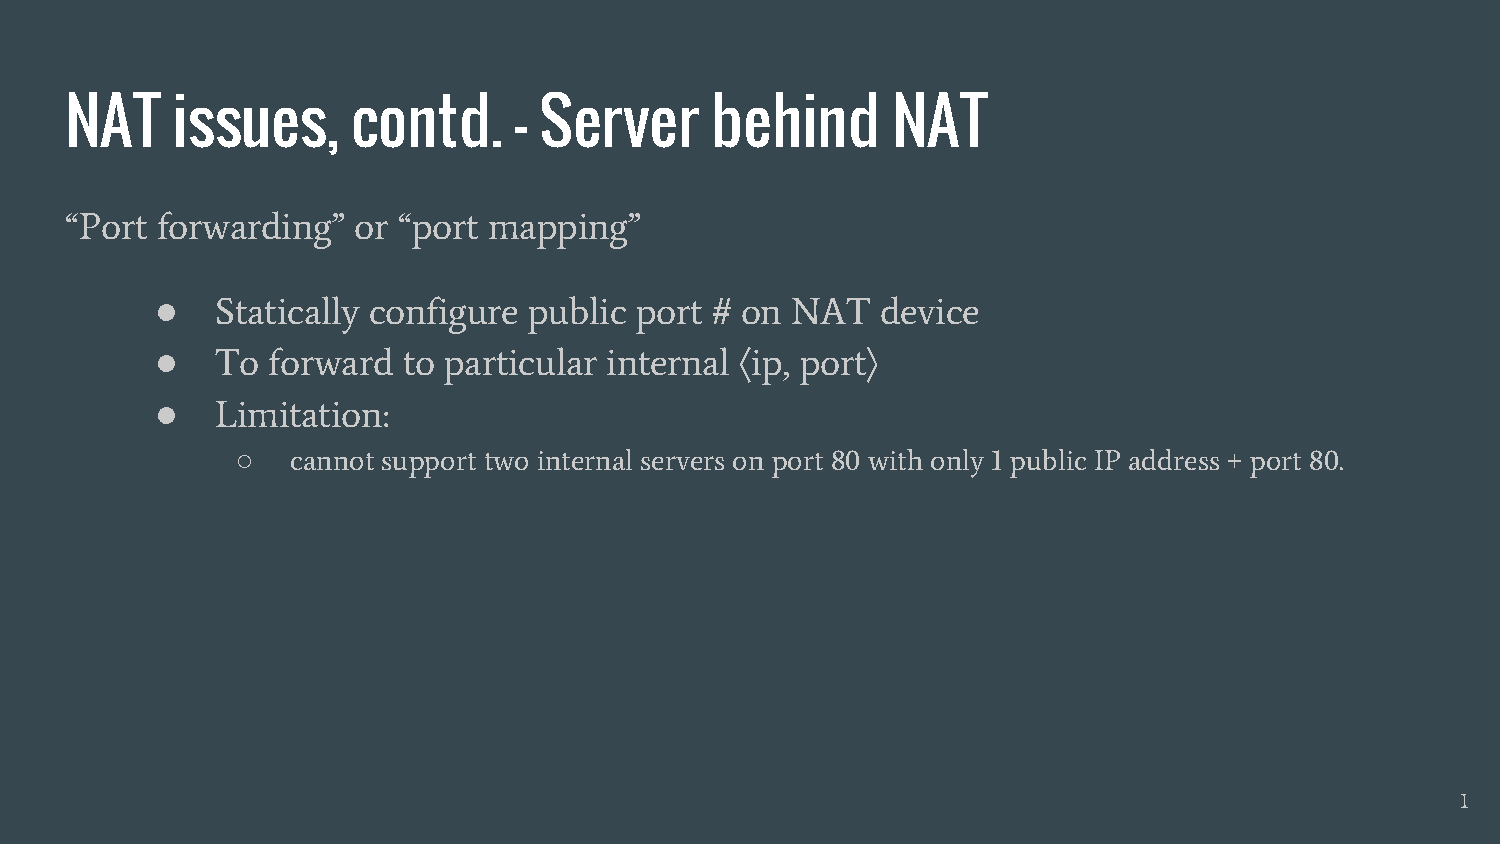
\includepdf[pages=1]{slides}
You basically map a specific port for that server (usually 80) on the NAT.

\includepdf[pages=2]{slides}
MISSED THIS, GOOGLE IT

\includepdf[pages=3]{slides}
Basically you have a server that sits outside and helps clients deal with NAT problems and such. Helps to determin the IP and port is allocated. Can also be used as a heartbeat type thing. 

\includepdf[pages=4]{slides}
Traversal Using Relays around NAT. This is kind of an alternative to STUM. It is meant to help you deal with troublesome NATS that perform address/port dependent mapping. This makes it hard to work with.

\includepdf[pages=5]{slides}
There are 2 NAT devices and a TURN client. There is a TURN server that is helping route between two peers. The TURN client has a private ip address that is NATed by the device, The client reserves an allocation at the TURN server for a relayed transport address. The TURN client is enabling other peers to send it packets on this new public address. This address is owned by the server and allocated to the client and packets will be forwarded there. If the TURN client wants to send packets to a peer it encapsulates the packets with a server transport address and sends them to the server for routing. The address of the peer the client is sending to is called the server reflexive transport address. This address is the address that the server would see (if the device is NATed the NATed address is used, else its standard ip address).   

\includepdf[pages=6]{slides}
The destination on the packet should first be the address and port of the TURN server. Once it gets there it removes a layer and looks at the TURN packet with now has its destination as the server reflexive address of the peer it actually wants to go to. The source address is the relayed transport address of the server. 

\includepdf[pages=7]{slides}
This shows the reason that endpoint independent behavior is favorable so that people can send data to your server easily. 

\includepdf[pages=8]{slides}




\end{document}